% Options for packages loaded elsewhere
\PassOptionsToPackage{unicode}{hyperref}
\PassOptionsToPackage{hyphens}{url}
%
\documentclass[
]{article}
\usepackage{amsmath,amssymb}
\usepackage{lmodern}
\usepackage{iftex}
\ifPDFTeX
  \usepackage[T1]{fontenc}
  \usepackage[utf8]{inputenc}
  \usepackage{textcomp} % provide euro and other symbols
\else % if luatex or xetex
  \usepackage{unicode-math}
  \defaultfontfeatures{Scale=MatchLowercase}
  \defaultfontfeatures[\rmfamily]{Ligatures=TeX,Scale=1}
\fi
% Use upquote if available, for straight quotes in verbatim environments
\IfFileExists{upquote.sty}{\usepackage{upquote}}{}
\IfFileExists{microtype.sty}{% use microtype if available
  \usepackage[]{microtype}
  \UseMicrotypeSet[protrusion]{basicmath} % disable protrusion for tt fonts
}{}
\makeatletter
\@ifundefined{KOMAClassName}{% if non-KOMA class
  \IfFileExists{parskip.sty}{%
    \usepackage{parskip}
  }{% else
    \setlength{\parindent}{0pt}
    \setlength{\parskip}{6pt plus 2pt minus 1pt}}
}{% if KOMA class
  \KOMAoptions{parskip=half}}
\makeatother
\usepackage{xcolor}
\usepackage[margin=1in]{geometry}
\usepackage{longtable,booktabs,array}
\usepackage{calc} % for calculating minipage widths
% Correct order of tables after \paragraph or \subparagraph
\usepackage{etoolbox}
\makeatletter
\patchcmd\longtable{\par}{\if@noskipsec\mbox{}\fi\par}{}{}
\makeatother
% Allow footnotes in longtable head/foot
\IfFileExists{footnotehyper.sty}{\usepackage{footnotehyper}}{\usepackage{footnote}}
\makesavenoteenv{longtable}
\usepackage{graphicx}
\makeatletter
\def\maxwidth{\ifdim\Gin@nat@width>\linewidth\linewidth\else\Gin@nat@width\fi}
\def\maxheight{\ifdim\Gin@nat@height>\textheight\textheight\else\Gin@nat@height\fi}
\makeatother
% Scale images if necessary, so that they will not overflow the page
% margins by default, and it is still possible to overwrite the defaults
% using explicit options in \includegraphics[width, height, ...]{}
\setkeys{Gin}{width=\maxwidth,height=\maxheight,keepaspectratio}
% Set default figure placement to htbp
\makeatletter
\def\fps@figure{htbp}
\makeatother
\setlength{\emergencystretch}{3em} % prevent overfull lines
\providecommand{\tightlist}{%
  \setlength{\itemsep}{0pt}\setlength{\parskip}{0pt}}
\setcounter{secnumdepth}{-\maxdimen} % remove section numbering
\ifLuaTeX
  \usepackage{selnolig}  % disable illegal ligatures
\fi
\IfFileExists{bookmark.sty}{\usepackage{bookmark}}{\usepackage{hyperref}}
\IfFileExists{xurl.sty}{\usepackage{xurl}}{} % add URL line breaks if available
\urlstyle{same} % disable monospaced font for URLs
\hypersetup{
  pdftitle={Resolução - Tarefa 3 (Regressão)},
  pdfauthor={Simone Kraievski Nadolny},
  hidelinks,
  pdfcreator={LaTeX via pandoc}}

\title{Resolução - Tarefa 3 (Regressão)}
\author{Simone Kraievski Nadolny}
\date{Última versão em 19/07/22}

\begin{document}
\maketitle

{
\setcounter{tocdepth}{2}
\tableofcontents
}
\hypertarget{machine-learning-em-r}{%
\section{Machine Learning em R}\label{machine-learning-em-r}}

\hypertarget{muxe9todos-supervisionados-de-regressuxe3o}{%
\subsection{Métodos Supervisionados de
Regressão}\label{muxe9todos-supervisionados-de-regressuxe3o}}

Nesta terceira tarefa usaremos um dataset relacionado com o serviço de
aluguel de bikes em DC, EUA, com registros por hora de aluguel de bikes
para o período 2011 a 2012.

\#Sobre o aluguel de Bikes em DC, EUA

Os sistemas de compartilhamento de bicicletas são a nova geração de
sistemas tradicionais de aluguel de bicicletas onde todo o processo de
adesão, aluguel e retorno se tornou automático. Através destes sistemas,
o usuário é capaz de alugar facilmente uma bicicleta de uma determinada
posição e retornar em outra posição. Atualmente, existem cerca de 500
programas de compartilhamento de bicicletas em todo o mundo, que é
composto de mais de 500 mil bicicletas. Hoje, existe um grande interesse
nestes sistemas devido ao seu importante papel em questões de tráfego,
meio ambiente e saúde.

Além das aplicações interessantes no mundo real dos sistemas de aluguel
de bicicletas, as características dos dados gerados por estes sistemas
os tornam atraentes para a pesquisa. Ao contrário de outros serviços de
transporte, como ônibus ou metrô, a duração da viagem, posição de
partida e chegada é explicitamente registrada nestes sistemas. Esta
característica transforma o sistema de compartilhamento de bicicletas em
uma rede virtual de sensores que pode ser usada para a detecção da
mobilidade na cidade. Portanto, espera-se que a maioria dos eventos
importantes na cidade possam ser detectados através do monitoramento
destes dados.

\hypertarget{dados}{%
\subsection{Dados}\label{dados}}

Os dados incluem contagens por hora do aluguel de bicicletas (por
membros e usuários casuais) da ``Capital Bikeshare'' em Washington, DC
entre 2011 e 2012, bem como informações meteorológicas sobre esses dias.

Você pode baixar os dados no link abaixo:
\url{https://archive.ics.uci.edu/ml/machine-learning-databases/00275/Bike-Sharing-Dataset.zip}

As fontes de dados originais se encontram em: -
\url{http://capitalbikeshare.com/system-data} -
\url{http://www.freemeteo.com}

O dataset chama-se ``hour.csv''. A descrição de cada uma das variáveis
pode ser encontrada no arquivo de ajuda do dataset, que pode ser
acessado executando ``?dcbikeshare'' em seu Console.

Para poder trabalhar com os dados, inicialmente sera adicionada as
bibliotecas iniciais e lido o arquivo.

\hypertarget{pergunta-1}{%
\section{Pergunta 1}\label{pergunta-1}}

Recodificar a variável season para um fator com nomes mais
significativos para cada nível: Recodificando a ``primavera'' (spring)
como categoria base. Dados: 1 - winter (inverno) 2 - spring (primavera)
3 - summer (verão) 4 - fall (outono)

\hypertarget{resposta-1}{%
\subsection{Resposta 1}\label{resposta-1}}

\hypertarget{pergunta-2}{%
\section{Pergunta 2}\label{pergunta-2}}

Recodificar as variáveis binárias holiday e workingday para serem
fatores Níveis: 0 - no (não) 1 - yes (sim)

Considere no como categoria base.

\hypertarget{resposta-2}{%
\subsection{Resposta 2}\label{resposta-2}}

\hypertarget{pergunta-3}{%
\section{Pergunta 3}\label{pergunta-3}}

Recodificar a variável yr para ser um fator com níveis Níveis: 0 - 2011
1 - 2012,

Considere 2011 como categoria base.

\hypertarget{resposta-3}{%
\subsection{Resposta 3}\label{resposta-3}}

\hypertarget{pergunta-4}{%
\section{Pergunta 4}\label{pergunta-4}}

Recodifique a variável weathersit para factor Níveis: 1 - claro 2 -
névoa 3 - precip leve 4 - precip pesada

Considerando claro como categoria base.

\hypertarget{resposta-4}{%
\subsection{Resposta 4}\label{resposta-4}}

\hypertarget{pergunta-5}{%
\section{Pergunta 5}\label{pergunta-5}}

Crie novas variáveis para as variáveis temperatura (temp), sensação
térmica (atemp), umidade (hum) e velocidade do vendo (windspeed)
calculando os valores brutos. As colunas temperatura (temp), sensação
térmica (atemp), umidade (hum) e velocidade do vento (windspeed) estão
normalizadas (0-1). - temp: para converter a graus Celsius multiplique
por 41 (valor máximo) - atemp: idem anterior, multiplique por 50 (valor
máximo) - hum: multiplique por 100 (valor máximo) - windspeed:
multiplique por 67 (valor máximo)

\hypertarget{resposta-5}{%
\subsection{Resposta 5}\label{resposta-5}}

\hypertarget{pergunta-6}{%
\section{Pergunta 6}\label{pergunta-6}}

Recodifique a variavel weekday para factor Níveis: 1: 2a-f 2: 3a-f 3:
4a-f 4: 5a-f 5: 6a-f 6: sábado 0: domingo (na tarefa estava dizendo que
domingo era o 7, porém não existia 7 nos dados e existia 0, então foi
usado 0 como domingo)

Considerando 2a-f como categoria base.

\hypertarget{resposta-6}{%
\subsection{Resposta 6}\label{resposta-6}}

\hypertarget{pergunta-7}{%
\section{Pergunta 7}\label{pergunta-7}}

Recodifique as variáveis hr para factor e mnth para factor. hr factor
com 24 níveis (de 0 a 23) e mnth para factor com 12 níveis (janeiro a
dezembro).

\hypertarget{resposta-7}{%
\subsection{Resposta 7}\label{resposta-7}}

\hypertarget{pergunta-8}{%
\section{Pergunta 8}\label{pergunta-8}}

Recrie visualização a seguir, e interprete-a no contexto dos dados.
Dica: Você precisará usar uma das variáveis que você criou acima. A
temperatura plotada é a sensação térmica. Antes de realizar o gráfico
verifique que o tipo da variável dteday deve ser Date e não chr.

\begin{figure}
\centering
\includegraphics{https://eps7008ufsc.netlify.app/Tarefa3_DCbike_files/figure-html/unnamed-chunk-9-1.png}
\caption{Imagem base}
\end{figure}

\hypertarget{resposta-8}{%
\subsection{Resposta 8}\label{resposta-8}}

Verificando se a variavel dteday está em formato de data:

\begin{verbatim}
## [1] "Date"
\end{verbatim}

Como ela está em formato de ``Date'' já pode-se começar a plotar o
gráfico solicitado
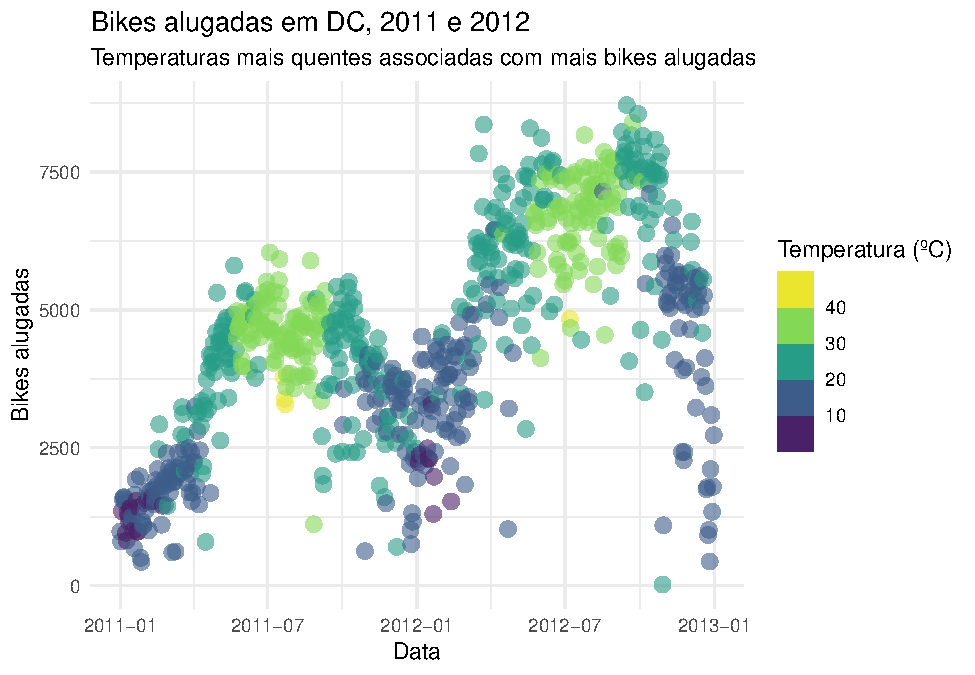
\includegraphics{Tarefa3Simone1_files/figure-latex/unnamed-chunk-10-1.pdf}

\hypertarget{pergunta-9}{%
\section{Pergunta 9}\label{pergunta-9}}

Recrie a visualização abaixo, mostrando a relação entre o aluguel de
bicicletas e a estação do ano (season). Interprete-a no contexto dos
dados.
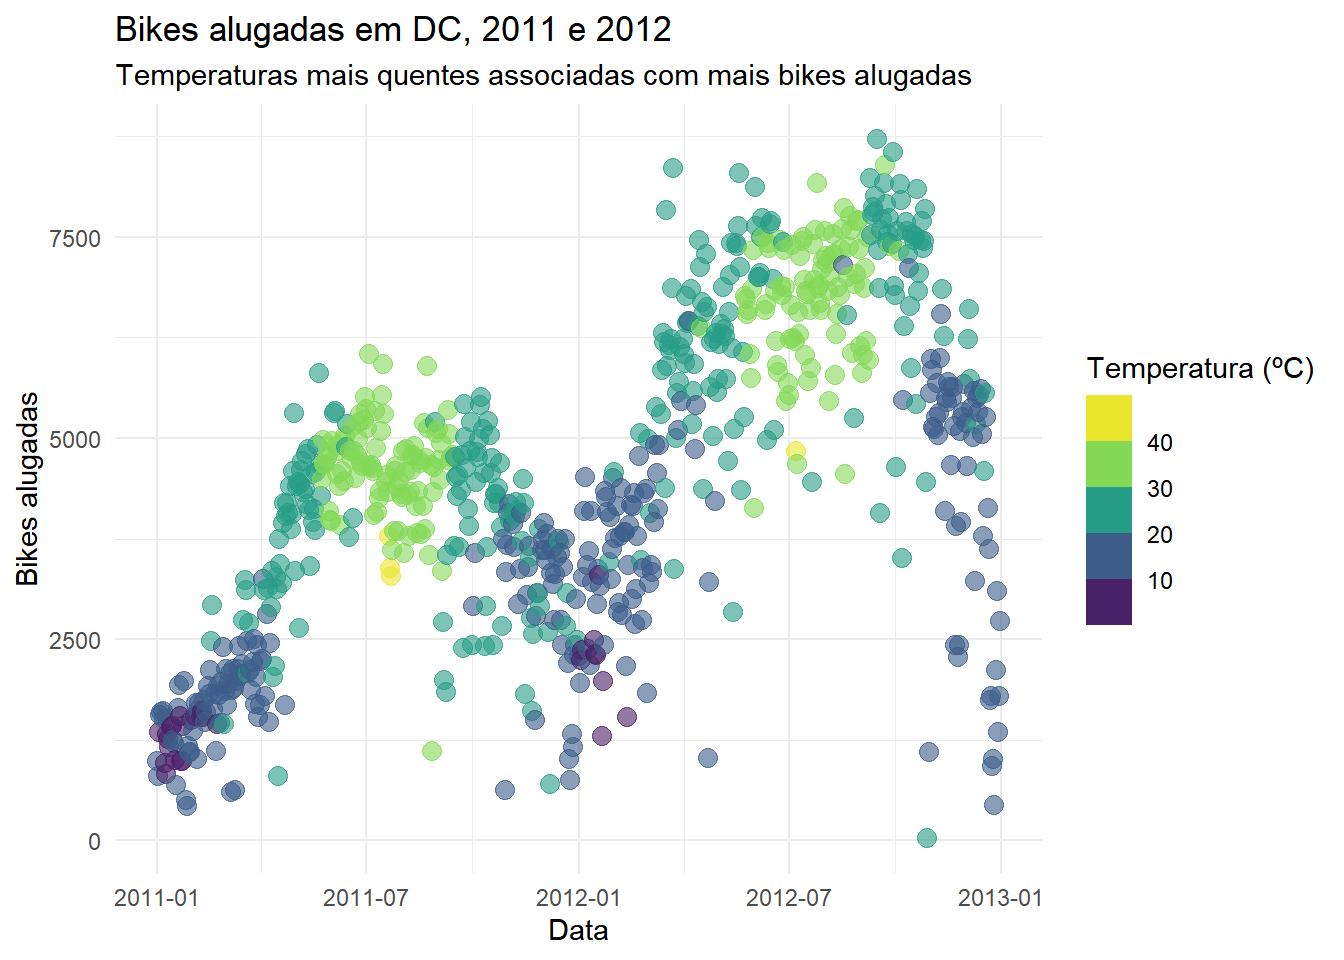
\includegraphics{https://eps7008ufsc.netlify.app/Tarefa3_DCbike_files/figure-html/unnamed-chunk-10-1.png}

\hypertarget{resposta-9}{%
\subsection{Resposta 9}\label{resposta-9}}

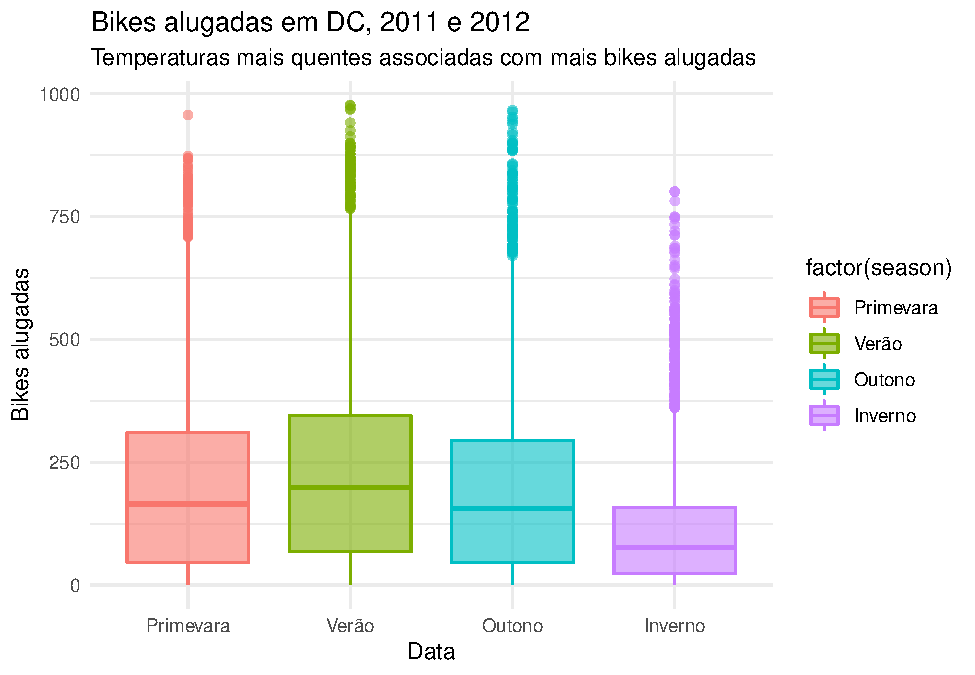
\includegraphics{Tarefa3Simone1_files/figure-latex/unnamed-chunk-11-1.pdf}

\hypertarget{pergunta-10}{%
\section{Pergunta 10}\label{pergunta-10}}

Separe o dataset em dois grupos, treinamento e teste, sendo a proporção
75 e 25 respectivamente, use obrigatoriamente o tidymodels (escoha quais
atributos irá usar e quais não e justifique suas escolhas).

\hypertarget{resposta-10}{%
\subsection{Resposta 10}\label{resposta-10}}

Inicialmente é necessário fazer um filtro no data frame e adicionar as
bibliotecas necessárias, logo será retiradas algumas colunas que não
serão necessárias. A tabela inicial consta com os seguintes dados:

\begin{longtable}[]{@{}ll@{}}
\caption{Data summary}\tabularnewline
\toprule()
\endhead
Name & bike\_shared \\
Number of rows & 17379 \\
Number of columns & 17 \\
\_\_\_\_\_\_\_\_\_\_\_\_\_\_\_\_\_\_\_\_\_\_\_ & \\
Column type frequency: & \\
Date & 1 \\
factor & 8 \\
numeric & 8 \\
\_\_\_\_\_\_\_\_\_\_\_\_\_\_\_\_\_\_\_\_\_\_\_\_ & \\
Group variables & None \\
\bottomrule()
\end{longtable}

\textbf{Variable type: Date}

\begin{longtable}[]{@{}
  >{\raggedright\arraybackslash}p{(\columnwidth - 12\tabcolsep) * \real{0.1750}}
  >{\raggedleft\arraybackslash}p{(\columnwidth - 12\tabcolsep) * \real{0.1250}}
  >{\raggedleft\arraybackslash}p{(\columnwidth - 12\tabcolsep) * \real{0.1750}}
  >{\raggedright\arraybackslash}p{(\columnwidth - 12\tabcolsep) * \real{0.1375}}
  >{\raggedright\arraybackslash}p{(\columnwidth - 12\tabcolsep) * \real{0.1375}}
  >{\raggedright\arraybackslash}p{(\columnwidth - 12\tabcolsep) * \real{0.1375}}
  >{\raggedleft\arraybackslash}p{(\columnwidth - 12\tabcolsep) * \real{0.1125}}@{}}
\toprule()
\begin{minipage}[b]{\linewidth}\raggedright
skim\_variable
\end{minipage} & \begin{minipage}[b]{\linewidth}\raggedleft
n\_missing
\end{minipage} & \begin{minipage}[b]{\linewidth}\raggedleft
complete\_rate
\end{minipage} & \begin{minipage}[b]{\linewidth}\raggedright
min
\end{minipage} & \begin{minipage}[b]{\linewidth}\raggedright
max
\end{minipage} & \begin{minipage}[b]{\linewidth}\raggedright
median
\end{minipage} & \begin{minipage}[b]{\linewidth}\raggedleft
n\_unique
\end{minipage} \\
\midrule()
\endhead
dteday & 0 & 1 & 2011-01-01 & 2012-12-31 & 2012-01-02 & 731 \\
\bottomrule()
\end{longtable}

\textbf{Variable type: factor}

\begin{longtable}[]{@{}
  >{\raggedright\arraybackslash}p{(\columnwidth - 10\tabcolsep) * \real{0.1429}}
  >{\raggedleft\arraybackslash}p{(\columnwidth - 10\tabcolsep) * \real{0.1020}}
  >{\raggedleft\arraybackslash}p{(\columnwidth - 10\tabcolsep) * \real{0.1429}}
  >{\raggedright\arraybackslash}p{(\columnwidth - 10\tabcolsep) * \real{0.0816}}
  >{\raggedleft\arraybackslash}p{(\columnwidth - 10\tabcolsep) * \real{0.0918}}
  >{\raggedright\arraybackslash}p{(\columnwidth - 10\tabcolsep) * \real{0.4388}}@{}}
\toprule()
\begin{minipage}[b]{\linewidth}\raggedright
skim\_variable
\end{minipage} & \begin{minipage}[b]{\linewidth}\raggedleft
n\_missing
\end{minipage} & \begin{minipage}[b]{\linewidth}\raggedleft
complete\_rate
\end{minipage} & \begin{minipage}[b]{\linewidth}\raggedright
ordered
\end{minipage} & \begin{minipage}[b]{\linewidth}\raggedleft
n\_unique
\end{minipage} & \begin{minipage}[b]{\linewidth}\raggedright
top\_counts
\end{minipage} \\
\midrule()
\endhead
season & 0 & 1 & FALSE & 4 & Ver: 4496, Pri: 4409, Inv: 4242, Out:
4232 \\
yr & 0 & 1 & FALSE & 2 & 202: 8734, 201: 8645 \\
mnth & 0 & 1 & FALSE & 12 & Mai: 1488, Jul: 1488, Dez: 1483, Ago:
1475 \\
hr & 0 & 1 & FALSE & 24 & 16: 730, 17: 730, 13: 729, 14: 729 \\
holiday & 0 & 1 & FALSE & 2 & Não: 16879, Sim: 500 \\
weekday & 0 & 1 & FALSE & 7 & Sáb: 2512, Dom: 2502, 6a-: 2487, 2a-:
2479 \\
workingday & 0 & 1 & FALSE & 2 & Sim: 11865, Não: 5514 \\
weathersit & 0 & 1 & FALSE & 4 & Cla: 11413, Név: 4544, Pre: 1419, Pre:
3 \\
\bottomrule()
\end{longtable}

\textbf{Variable type: numeric}

\begin{longtable}[]{@{}
  >{\raggedright\arraybackslash}p{(\columnwidth - 20\tabcolsep) * \real{0.1458}}
  >{\raggedleft\arraybackslash}p{(\columnwidth - 20\tabcolsep) * \real{0.1042}}
  >{\raggedleft\arraybackslash}p{(\columnwidth - 20\tabcolsep) * \real{0.1458}}
  >{\raggedleft\arraybackslash}p{(\columnwidth - 20\tabcolsep) * \real{0.0833}}
  >{\raggedleft\arraybackslash}p{(\columnwidth - 20\tabcolsep) * \real{0.0833}}
  >{\raggedleft\arraybackslash}p{(\columnwidth - 20\tabcolsep) * \real{0.0521}}
  >{\raggedleft\arraybackslash}p{(\columnwidth - 20\tabcolsep) * \real{0.0833}}
  >{\raggedleft\arraybackslash}p{(\columnwidth - 20\tabcolsep) * \real{0.0833}}
  >{\raggedleft\arraybackslash}p{(\columnwidth - 20\tabcolsep) * \real{0.0938}}
  >{\raggedleft\arraybackslash}p{(\columnwidth - 20\tabcolsep) * \real{0.0625}}
  >{\raggedright\arraybackslash}p{(\columnwidth - 20\tabcolsep) * \real{0.0625}}@{}}
\toprule()
\begin{minipage}[b]{\linewidth}\raggedright
skim\_variable
\end{minipage} & \begin{minipage}[b]{\linewidth}\raggedleft
n\_missing
\end{minipage} & \begin{minipage}[b]{\linewidth}\raggedleft
complete\_rate
\end{minipage} & \begin{minipage}[b]{\linewidth}\raggedleft
mean
\end{minipage} & \begin{minipage}[b]{\linewidth}\raggedleft
sd
\end{minipage} & \begin{minipage}[b]{\linewidth}\raggedleft
p0
\end{minipage} & \begin{minipage}[b]{\linewidth}\raggedleft
p25
\end{minipage} & \begin{minipage}[b]{\linewidth}\raggedleft
p50
\end{minipage} & \begin{minipage}[b]{\linewidth}\raggedleft
p75
\end{minipage} & \begin{minipage}[b]{\linewidth}\raggedleft
p100
\end{minipage} & \begin{minipage}[b]{\linewidth}\raggedright
hist
\end{minipage} \\
\midrule()
\endhead
instant & 0 & 1 & 8690.00 & 5017.03 & 1.00 & 4345.50 & 8690.00 &
13034.50 & 17379 & ▇▇▇▇▇ \\
temp & 0 & 1 & 20.38 & 7.89 & 0.82 & 13.94 & 20.50 & 27.06 & 41 &
▂▇▇▇▁ \\
atemp & 0 & 1 & 23.79 & 8.59 & 0.00 & 16.66 & 24.24 & 31.06 & 50 &
▁▆▇▆▁ \\
hum & 0 & 1 & 62.72 & 19.29 & 0.00 & 48.00 & 63.00 & 78.00 & 100 &
▁▃▇▇▆ \\
windspeed & 0 & 1 & 12.74 & 8.20 & 0.00 & 7.00 & 13.00 & 17.00 & 57 &
▇▆▂▁▁ \\
casual & 0 & 1 & 35.68 & 49.31 & 0.00 & 4.00 & 17.00 & 48.00 & 367 &
▇▁▁▁▁ \\
registered & 0 & 1 & 153.79 & 151.36 & 0.00 & 34.00 & 115.00 & 220.00 &
886 & ▇▃▁▁▁ \\
cnt & 0 & 1 & 189.46 & 181.39 & 1.00 & 40.00 & 142.00 & 281.00 & 977 &
▇▃▁▁▁ \\
\bottomrule()
\end{longtable}

Após a análise dos tipos de dados pode ser interessante também uma
análise dos valores encontrados, que serão apresentados a seguir:

\begin{verbatim}
##     instant          dteday                 season        yr      
##  Min.   :    1   Min.   :2011-01-01   Primevara:4409   2011:8645  
##  1st Qu.: 4346   1st Qu.:2011-07-04   Verão    :4496   2021:8734  
##  Median : 8690   Median :2012-01-02   Outono   :4232              
##  Mean   : 8690   Mean   :2012-01-02   Inverno  :4242              
##  3rd Qu.:13034   3rd Qu.:2012-07-02                               
##  Max.   :17379   Max.   :2012-12-31                               
##                                                                   
##        mnth            hr        holiday        weekday     workingday 
##  Maio    :1488   16     :  730   Não:16879   2a-f   :2479   Não: 5514  
##  Julho   :1488   17     :  730   Sim:  500   3a-fa  :2453   Sim:11865  
##  Dezembro:1483   13     :  729               4a-f   :2475              
##  Agosto  :1475   14     :  729               5a-f   :2471              
##  Março   :1473   15     :  729               6a-f   :2487              
##  Outubro :1451   12     :  728               Sábado :2512              
##  (Other) :8521   (Other):13004               Domingo:2502              
##           weathersit         temp           atemp            hum        
##  Claro         :11413   Min.   : 0.82   Min.   : 0.00   Min.   :  0.00  
##  Névoa         : 4544   1st Qu.:13.94   1st Qu.:16.66   1st Qu.: 48.00  
##  Precip. leve  : 1419   Median :20.50   Median :24.24   Median : 63.00  
##  Precip. pesada:    3   Mean   :20.38   Mean   :23.79   Mean   : 62.72  
##                         3rd Qu.:27.06   3rd Qu.:31.06   3rd Qu.: 78.00  
##                         Max.   :41.00   Max.   :50.00   Max.   :100.00  
##                                                                         
##    windspeed          casual         registered         cnt       
##  Min.   : 0.000   Min.   :  0.00   Min.   :  0.0   Min.   :  1.0  
##  1st Qu.: 7.002   1st Qu.:  4.00   1st Qu.: 34.0   1st Qu.: 40.0  
##  Median :12.998   Median : 17.00   Median :115.0   Median :142.0  
##  Mean   :12.737   Mean   : 35.68   Mean   :153.8   Mean   :189.5  
##  3rd Qu.:16.998   3rd Qu.: 48.00   3rd Qu.:220.0   3rd Qu.:281.0  
##  Max.   :56.997   Max.   :367.00   Max.   :886.0   Max.   :977.0  
## 
\end{verbatim}

\begin{verbatim}
## 
## Call:
## lm(formula = cnt ~ ., data = bike_shared)
## 
## Residuals:
##        Min         1Q     Median         3Q        Max 
## -6.298e-11 -9.000e-14  1.000e-14  1.000e-13  3.843e-10 
## 
## Coefficients: (1 not defined because of singularities)
##                            Estimate Std. Error    t value Pr(>|t|)    
## (Intercept)               5.368e-09  7.558e-10  7.103e+00 1.27e-12 ***
## instant                   1.492e-14  2.114e-15  7.060e+00 1.73e-12 ***
## dteday                   -3.582e-13  5.046e-14 -7.098e+00 1.31e-12 ***
## seasonVerão              -9.103e-14  1.517e-13 -6.000e-01 0.548546    
## seasonOutono             -5.718e-13  1.752e-13 -3.263e+00 0.001106 ** 
## seasonInverno            -6.246e-13  1.483e-13 -4.212e+00 2.55e-05 ***
## yr2021                    1.278e-12  9.851e-13  1.297e+00 0.194612    
## mnthFevereiro            -3.986e-13  1.485e-13 -2.684e+00 0.007284 ** 
## mnthMarço                -2.104e-13  2.130e-13 -9.880e-01 0.323309    
## mnthAbril                -2.669e-14  3.128e-13 -8.500e-02 0.932013    
## mnthMaio                 -4.267e-13  3.832e-13 -1.114e+00 0.265476    
## mnthJunho                -7.452e-14  4.550e-13 -1.640e-01 0.869909    
## mnthJulho                -1.281e-13  5.393e-13 -2.380e-01 0.812203    
## mnthAgosto               -5.844e-14  6.116e-13 -9.600e-02 0.923878    
## mnthSetembro              8.427e-14  6.819e-13  1.240e-01 0.901652    
## mnthOutubro               1.187e-12  7.609e-13  1.560e+00 0.118802    
## mnthNovembro              1.121e-12  8.416e-13  1.332e+00 0.182852    
## mnthDezembro              1.289e-12  9.129e-13  1.412e+00 0.158004    
## hr1                      -9.661e-13  1.628e-13 -5.933e+00 3.04e-09 ***
## hr2                       5.539e-13  1.635e-13  3.388e+00 0.000707 ***
## hr3                      -1.395e-12  1.649e-13 -8.461e+00  < 2e-16 ***
## hr4                       1.535e-12  1.652e-13  9.291e+00  < 2e-16 ***
## hr5                      -1.084e-12  1.640e-13 -6.609e+00 3.97e-11 ***
## hr6                      -1.911e-12  1.640e-13 -1.165e+01  < 2e-16 ***
## hr7                      -4.350e-13  1.703e-13 -2.555e+00 0.010626 *  
## hr8                       2.712e-13  1.841e-13  1.473e+00 0.140717    
## hr9                      -9.122e-13  1.684e-13 -5.417e+00 6.15e-08 ***
## hr10                     -9.060e-13  1.668e-13 -5.431e+00 5.69e-08 ***
## hr11                     -9.371e-13  1.695e-13 -5.529e+00 3.27e-08 ***
## hr12                     -9.537e-13  1.728e-13 -5.518e+00 3.48e-08 ***
## hr13                     -9.195e-13  1.742e-13 -5.279e+00 1.32e-07 ***
## hr14                     -1.093e-12  1.752e-13 -6.239e+00 4.52e-10 ***
## hr15                     -8.425e-13  1.759e-13 -4.788e+00 1.70e-06 ***
## hr16                     -6.974e-13  1.786e-13 -3.904e+00 9.49e-05 ***
## hr17                     -1.625e-12  1.922e-13 -8.451e+00  < 2e-16 ***
## hr18                     -2.266e-12  1.891e-13 -1.198e+01  < 2e-16 ***
## hr19                     -2.369e-12  1.779e-13 -1.331e+01  < 2e-16 ***
## hr20                     -7.308e-13  1.726e-13 -4.234e+00 2.31e-05 ***
## hr21                      1.614e-15  1.704e-13  9.000e-03 0.992446    
## hr22                     -3.057e-13  1.697e-13 -1.801e+00 0.071691 .  
## hr23                     -2.590e-13  1.696e-13 -1.527e+00 0.126757    
## holidaySim               -1.168e-13  1.509e-13 -7.740e-01 0.438771    
## weekday3a-fa              8.015e-14  9.066e-14  8.840e-01 0.376640    
## weekday4a-f               6.501e-14  9.060e-14  7.170e-01 0.473080    
## weekday5a-f               7.721e-14  9.033e-14  8.550e-01 0.392654    
## weekday6a-f               3.725e-14  9.024e-14  4.130e-01 0.679745    
## weekdaySábado             1.382e-13  9.665e-14  1.430e+00 0.152769    
## weekdayDomingo            4.119e-14  9.592e-14  4.290e-01 0.667614    
## workingdaySim                    NA         NA         NA       NA    
## weathersitNévoa          -1.123e-13  5.855e-14 -1.918e+00 0.055159 .  
## weathersitPrecip. leve   -5.083e-13  9.973e-14 -5.097e+00 3.49e-07 ***
## weathersitPrecip. pesada -9.288e-13  1.794e-12 -5.180e-01 0.604583    
## temp                      4.422e-14  2.200e-14  2.010e+00 0.044399 *  
## atemp                    -1.470e-14  1.868e-14 -7.870e-01 0.431157    
## hum                       4.593e-15  1.711e-15  2.684e+00 0.007277 ** 
## windspeed                -4.411e-15  3.211e-15 -1.374e+00 0.169518    
## casual                    1.000e+00  8.052e-16  1.242e+15  < 2e-16 ***
## registered                1.000e+00  2.979e-16  3.356e+15  < 2e-16 ***
## ---
## Signif. codes:  0 '***' 0.001 '**' 0.01 '*' 0.05 '.' 0.1 ' ' 1
## 
## Residual standard error: 3.098e-12 on 17322 degrees of freedom
## Multiple R-squared:      1,  Adjusted R-squared:      1 
## F-statistic: 1.064e+30 on 56 and 17322 DF,  p-value: < 2.2e-16
\end{verbatim}

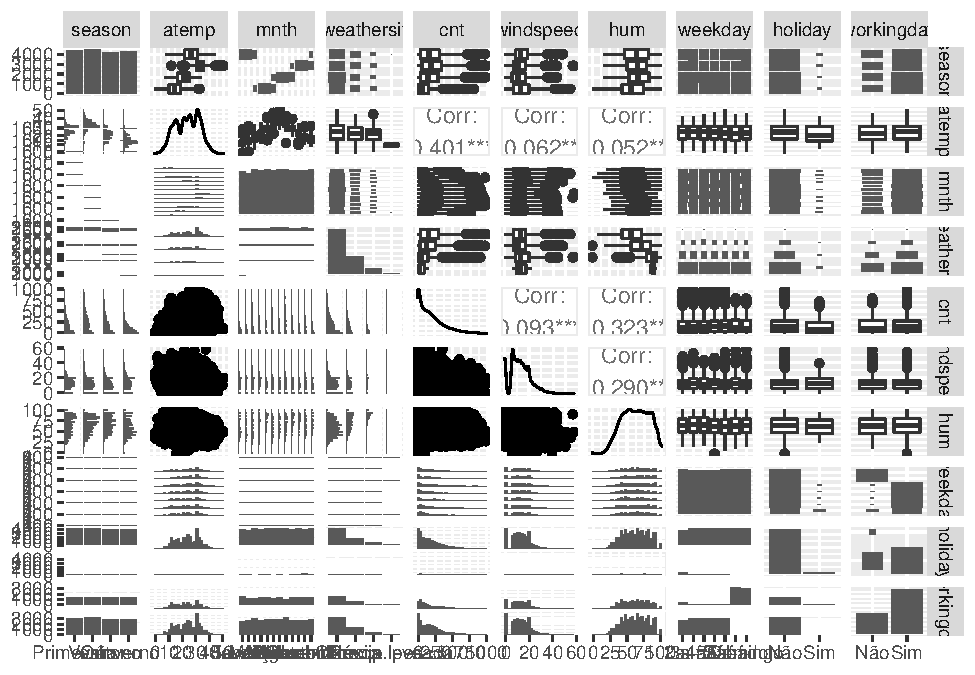
\includegraphics{Tarefa3Simone1_files/figure-latex/unnamed-chunk-15-1.pdf}

Das 17 colunas apresentadas, podemos desconsiderar para as análises a
``instant'', ``yr'' visto que só existem dois factores e existe a
variável ``dteday'', mês e hora serão mantidas para facilitar análises
mais sazonais, também não será inclusa nas análises o ``temp'' visto que
o atemp já irá substituir essa variável que oferece informações
semelhantes, ``hum'' e ``windspeed'' não entraram nas análises, também
não entrará o ``casual'' ou o ``registered'' visto que esses dois dados
já estão inclusos na sua soma em cnt.

\hypertarget{pergunta-11}{%
\section{Pergunta 11}\label{pergunta-11}}

Crie um objeto de validação cruzada, com k=10 usando tidymodels, mostre
o código. Use este objeto para todas as questões a seguir.

\hypertarget{resposta-11}{%
\subsection{Resposta 11}\label{resposta-11}}

\hypertarget{pergunta-12}{%
\section{Pergunta 12}\label{pergunta-12}}

Ajuste um modelo linear prevendo o total de aluguéis de bicicletas a
partir dos atributos presentes no dataset. Calcule o R2, o RMSE e o MAE.

\hypertarget{resposta-12}{%
\subsection{Resposta 12}\label{resposta-12}}

\begin{verbatim}
## # A tibble: 3 x 6
##   .metric .estimator    mean     n std_err .config             
##   <chr>   <chr>        <dbl> <int>   <dbl> <chr>               
## 1 mae     standard    75.4      10 0.798   Preprocessor1_Model1
## 2 rmse    standard   102.       10 0.934   Preprocessor1_Model1
## 3 rsq     standard     0.684    10 0.00328 Preprocessor1_Model1
\end{verbatim}

\hypertarget{pergunta-13}{%
\section{Pergunta 13}\label{pergunta-13}}

Ajuste um modelo de árvore de decisão prevendo o total de aluguéis de
bicicletas a partir dos atributos presentes no dataset. Calcule o R2, o
RMSE e o MAE.

\hypertarget{resposta-13}{%
\subsection{Resposta 13}\label{resposta-13}}

\begin{verbatim}
## # A tibble: 3 x 6
##   .metric .estimator    mean     n std_err .config             
##   <chr>   <chr>        <dbl> <int>   <dbl> <chr>               
## 1 mae     standard    94.3      10 0.670   Preprocessor1_Model1
## 2 rmse    standard   125.       10 1.14    Preprocessor1_Model1
## 3 rsq     standard     0.527    10 0.00912 Preprocessor1_Model1
\end{verbatim}

\hypertarget{pergunta-14}{%
\section{Pergunta 14}\label{pergunta-14}}

Utilize o algoritmo Random Forests para prever o total de aluguéis de
bicicletas a partir dos atributos presentes no dataset. Calcule o R2, o
RMSE e o MAE.

\hypertarget{resposta-14}{%
\subsection{Resposta 14}\label{resposta-14}}

\begin{verbatim}
## # A tibble: 3 x 6
##   .metric .estimator   mean     n std_err .config             
##   <chr>   <chr>       <dbl> <int>   <dbl> <chr>               
## 1 mae     standard   41.9      10 0.342   Preprocessor1_Model1
## 2 rmse    standard   62.0      10 0.558   Preprocessor1_Model1
## 3 rsq     standard    0.895    10 0.00202 Preprocessor1_Model1
\end{verbatim}

\hypertarget{pergunta-15}{%
\section{Pergunta 15}\label{pergunta-15}}

Qual dos três modelos foi melhor? Dica: compare os R2, os RMSE e os MAE
usando uma tabela.

\hypertarget{resposta-15}{%
\subsection{Resposta 15}\label{resposta-15}}

\includegraphics{Tarefa3Simone1_files/figure-latex/unnamed-chunk-21-1.pdf}
Assim, o melhor modelo é o do Random Forests

\begin{verbatim}
## # A tibble: 2 x 4
##   .metric .estimator .estimate .config             
##   <chr>   <chr>          <dbl> <chr>               
## 1 rmse    standard      63.0   Preprocessor1_Model1
## 2 rsq     standard       0.893 Preprocessor1_Model1
\end{verbatim}

\hypertarget{pergunta-16}{%
\section{Pergunta 16}\label{pergunta-16}}

Use o melhor modelo para calcular o R2, o RMSE e o MAE no dataset de
teste. Grafique o total de aluguéis (cnt) no eixo x e o valor estimado
no eixo y

\hypertarget{resposta-16}{%
\subsection{Resposta 16}\label{resposta-16}}

\includegraphics{Tarefa3Simone1_files/figure-latex/unnamed-chunk-23-1.pdf}

\begin{verbatim}
## Warning: `pull_workflow_fit()` was deprecated in workflows 0.2.3.
## Please use `extract_fit_parsnip()` instead.
\end{verbatim}

\includegraphics{Tarefa3Simone1_files/figure-latex/unnamed-chunk-24-1.pdf}

\end{document}
